\documentclass{standalone}
\usepackage{tikz}
\usetikzlibrary{positioning,calc}
\begin{document}
\begin{tikzpicture}
\tikzstyle{firing} = [fill=blue!40, rounded corners=3pt];
\tikzstyle{lbl} = [font=\small];


\draw[black!40] (0, 0) grid (60, 4); 

\draw[->, black, line width=1.5pt] (0, 0) -- (31, 0);
\draw[-, black, line width=1.5pt] (0, 0) -- (0, 4);
\foreach \i in {30,31,...,60} {
    \draw[black, line width=1pt] (\i, 0) -- +(0, -2.5pt);
    \node[below=4pt] at (\i-30, 0) {\i};
}

\draw[firing] (0, 1) rectangle (1, 2);
\node[lbl] at (0.5, 1.5) {c};
\draw[firing] (0, 2) rectangle (1, 3);
\node[lbl] at (0.5, 2.5) {c};
\draw[firing] (3, 1) rectangle (4, 2);
\node[lbl] at (3.5, 1.5) {c};
\draw[firing] (3, 2) rectangle (4, 3);
\node[lbl] at (3.5, 2.5) {c};
\draw[firing] (6, 1) rectangle (7, 2);
\node[lbl] at (6.5, 1.5) {c};
\draw[firing] (6, 2) rectangle (7, 3);
\node[lbl] at (6.5, 2.5) {c};
\draw[firing] (9, 1) rectangle (10, 2);
\node[lbl] at (9.5, 1.5) {c};
\draw[firing] (9, 2) rectangle (10, 3);
\node[lbl] at (9.5, 2.5) {c};
\draw[firing] (12, 0) rectangle (13, 1);
\node[lbl] at (12.5, 0.5) {c};
\draw[firing] (12, 1) rectangle (13, 2);
\node[lbl] at (12.5, 1.5) {c};
\draw[firing] (15, 1) rectangle (16, 2);
\node[lbl] at (15.5, 1.5) {c};
\draw[firing] (15, 2) rectangle (16, 3);
\node[lbl] at (15.5, 2.5) {c};
\draw[firing] (18, 1) rectangle (19, 2);
\node[lbl] at (18.5, 1.5) {c};
\draw[firing] (18, 2) rectangle (19, 3);
\node[lbl] at (18.5, 2.5) {c};
\draw[firing] (21, 0) rectangle (22, 1);
\node[lbl] at (21.5, 0.5) {c};
\draw[firing] (21, 1) rectangle (22, 2);
\node[lbl] at (21.5, 1.5) {c};
\draw[firing] (24, 1) rectangle (25, 2);
\node[lbl] at (24.5, 1.5) {c};
\draw[firing] (24, 2) rectangle (25, 3);
\node[lbl] at (24.5, 2.5) {c};
\draw[firing] (27, 1) rectangle (28, 2);
\node[lbl] at (27.5, 1.5) {c};
\draw[firing] (27, 2) rectangle (28, 3);
\node[lbl] at (27.5, 2.5) {c};
\draw[firing] (30, 0) rectangle (30, 1);
\node[lbl] at (30.5, 0.5) {c};
\draw[firing] (30, 1) rectangle (30, 2);
\node[lbl] at (30.5, 1.5) {c};
\draw[firing] (2, 0) rectangle (3, 1);
\node[lbl] at (2.5, 0.5) {b};
\draw[firing] (5, 0) rectangle (6, 1);
\node[lbl] at (5.5, 0.5) {b};
\draw[firing] (5, 2) rectangle (6, 3);
\node[lbl] at (5.5, 2.5) {b};
\draw[firing] (8, 0) rectangle (9, 1);
\node[lbl] at (8.5, 0.5) {b};
\draw[firing] (11, 0) rectangle (12, 1);
\node[lbl] at (11.5, 0.5) {b};
\draw[firing] (13, 0) rectangle (14, 1);
\node[lbl] at (13.5, 0.5) {b};
\draw[firing] (16, 0) rectangle (17, 1);
\node[lbl] at (16.5, 0.5) {b};
\draw[firing] (19, 0) rectangle (20, 1);
\node[lbl] at (19.5, 0.5) {b};
\draw[firing] (22, 0) rectangle (23, 1);
\node[lbl] at (22.5, 0.5) {b};
\draw[firing] (25, 0) rectangle (26, 1);
\node[lbl] at (25.5, 0.5) {b};
\draw[firing] (28, 0) rectangle (29, 1);
\node[lbl] at (28.5, 0.5) {b};
\draw[firing] (0, 0) rectangle (2, 1);
\node[lbl] at (1.0, 0.5) {a};
\draw[firing] (3, 0) rectangle (5, 1);
\node[lbl] at (4.0, 0.5) {a};
\draw[firing] (6, 0) rectangle (8, 1);
\node[lbl] at (7.0, 0.5) {a};
\draw[firing] (9, 0) rectangle (11, 1);
\node[lbl] at (10.0, 0.5) {a};
\draw[firing] (14, 0) rectangle (16, 1);
\node[lbl] at (15.0, 0.5) {a};
\draw[firing] (17, 0) rectangle (19, 1);
\node[lbl] at (18.0, 0.5) {a};
\draw[firing] (23, 0) rectangle (25, 1);
\node[lbl] at (24.0, 0.5) {a};
\draw[firing] (26, 0) rectangle (28, 1);
\node[lbl] at (27.0, 0.5) {a};
\draw[firing] (1, 1) rectangle (3, 2);
\node[lbl] at (2.0, 1.5) {d};
\draw[firing] (4, 1) rectangle (6, 2);
\node[lbl] at (5.0, 1.5) {d};
\draw[firing] (7, 1) rectangle (9, 2);
\node[lbl] at (8.0, 1.5) {d};
\draw[firing] (10, 1) rectangle (12, 2);
\node[lbl] at (11.0, 1.5) {d};
\draw[firing] (13, 1) rectangle (15, 2);
\node[lbl] at (14.0, 1.5) {d};
\draw[firing] (16, 1) rectangle (18, 2);
\node[lbl] at (17.0, 1.5) {d};
\draw[firing] (19, 1) rectangle (21, 2);
\node[lbl] at (20.0, 1.5) {d};
\draw[firing] (22, 1) rectangle (24, 2);
\node[lbl] at (23.0, 1.5) {d};
\draw[firing] (25, 1) rectangle (27, 2);
\node[lbl] at (26.0, 1.5) {d};
\draw[firing] (28, 1) rectangle (30, 2);
\node[lbl] at (29.0, 1.5) {d};
\end{tikzpicture}
\end{document}